\documentclass{article}
\usepackage{graphicx}
\usepackage{authblk}
\usepackage{amsmath}
\usepackage{listings}

\begin{document}


\title{THEORETICAL NEUROSCIENCE II \\ EXERCISE 04}
\date{10 Mai. 2013}
\author[1]{Yunus Emre Demiray, Taygun C. Uzuneser, \c{S}eyma Bayrak\thanks{seyma.bayrak@st.ovgu.de}}
\affil[1]{\footnotesize  Otto von Guericke University of Magdeburg}
\maketitle

\newpage

\section{Introduction: Associative Memory Patterns and Their Activation Function}
The activation function $F$ for the associative network is chosen to be saturative and rectified with a negative threshold $\gamma=-20$ as shown in equation 1.

\begin{equation}
 F(I)=150[tanh(\frac{I-\gamma}{150})]_+=F(I)=150[tanh(\frac{I+20}{150})]_+
\end{equation}

Each associative memory pattern (also called auto-associative memory) can be thought as a vector having $N_{mem}$ stored elements in it, such that $v^m$ with $m=1,2,3,...,N_{mem}$.

The auto associative network model is assumed to be similar to the recurrent network firing rate model given below.

\begin{equation}
 \tau_r \frac{d\textbf{v}}{dt}=-\textbf{v}+F(\textbf{h}+\textbf{M}.\textbf{v})
\end{equation}

The matrix $\textbf{M}$ denotes the recurrent synaptic interactions among the post-synaptic neurons at the same layer, this matrix reflects the strenght of their interactions. One important difference between recurrent model and associative network is that, the matrix $\textbf{h}$ is assumed to be $0$ in associative model. Since the associative recall is achieved by starting the network in an initial state that is almost proportional to $\textbf{v}(0)=c\textbf{v}^m$ ($c$ is a constent and $m$ is the index of vector), so the matrix $\textbf{h}=\textbf{W.u}$, which actually stands for the input vector and synaptic weight effects to the output vector \textbf{v}, can be assumed to be zero.$^{[1]}$


The weight matrix \textbf{M} is chosen as 

\begin{equation}
 M=\frac{\lambda \sum_{i=1}^{N_{mem}} (\textbf{v}^i -\alpha c \textbf{n}) (\textbf{v}^i -\alpha c \textbf{n})^T }{c^2 \alpha N_v (1-\alpha)} - \frac{\textbf{n} \textbf{n}^T}{\alpha N_v}
\end{equation}

where $N_{mem}$ is the number of memory pattern vector \textbf{v}, $N_{v}$ is the length of \textbf{v} (it means the number of stored data in one pattern), \textbf{n} is the unit vector having equal length to \textbf{v}, and $\alpha$ stands for the probability of assigning an activity to inside the pattern such that $N_v \alpha$. 

Let us look if the network activity pattern can have a fixed point. The condition is the activity to match with one of the memories e.g. \textbf{v}$=c'$\textbf{v}$^1$, then equation 2 turns out to be (with the assumption of $\textbf{h}=0$)

\begin{equation}
 c'\textbf{v}^1=F(c'\textbf{M.v}^1) \longrightarrow F(-c'(1+\alpha))=0 \;\;\;\;\; and \;\;\;\;\; F(c(\lambda-1-\alpha \lambda ))=c
\end{equation}

\section{Assignments}
\subsection{}

Show that the equation 4 stated in introduction part is satisfied for the given parameters $c=18.731$, $\alpha=0.25$ and $\lambda=1.25$.

\begin{equation*}
 F(-c(1+\alpha \lambda))=0 \;\;\;\;\;\;and \;\;\;\;\;\; c=F(c(\lambda-1-\alpha \lambda))
\end{equation*}

$\longrightarrow$ $ F(-c(1+\alpha \lambda))=F(-18,731(1+0,25.1,25))=F(-25,584)$ \newline

$=150[tanh(\frac{-25,584+20}{150})]_{+}=150[tanh(-0.031)]_+=0$ \;\;\;\;     qed \newline

$\longrightarrow F(c(\lambda-1-\alpha \lambda))=F(-18,731(1,25-1-0,25.1,25))=F(-1,171) $ \newline

$=150 [tanh(\frac{-1,171+20}{150})]_+=150[]_+=150[tanh(0.122)]_+=18.731=c$  \;\;\;\;     qed \newline

The provided MATLAB code \textit{memory.m} creates already 4 \textbf{v}$^N_{mem}$ patterns and it plots the following input pattern (or so called memory pattern) for the vector $v^1$ and its activity.

\begin{center}
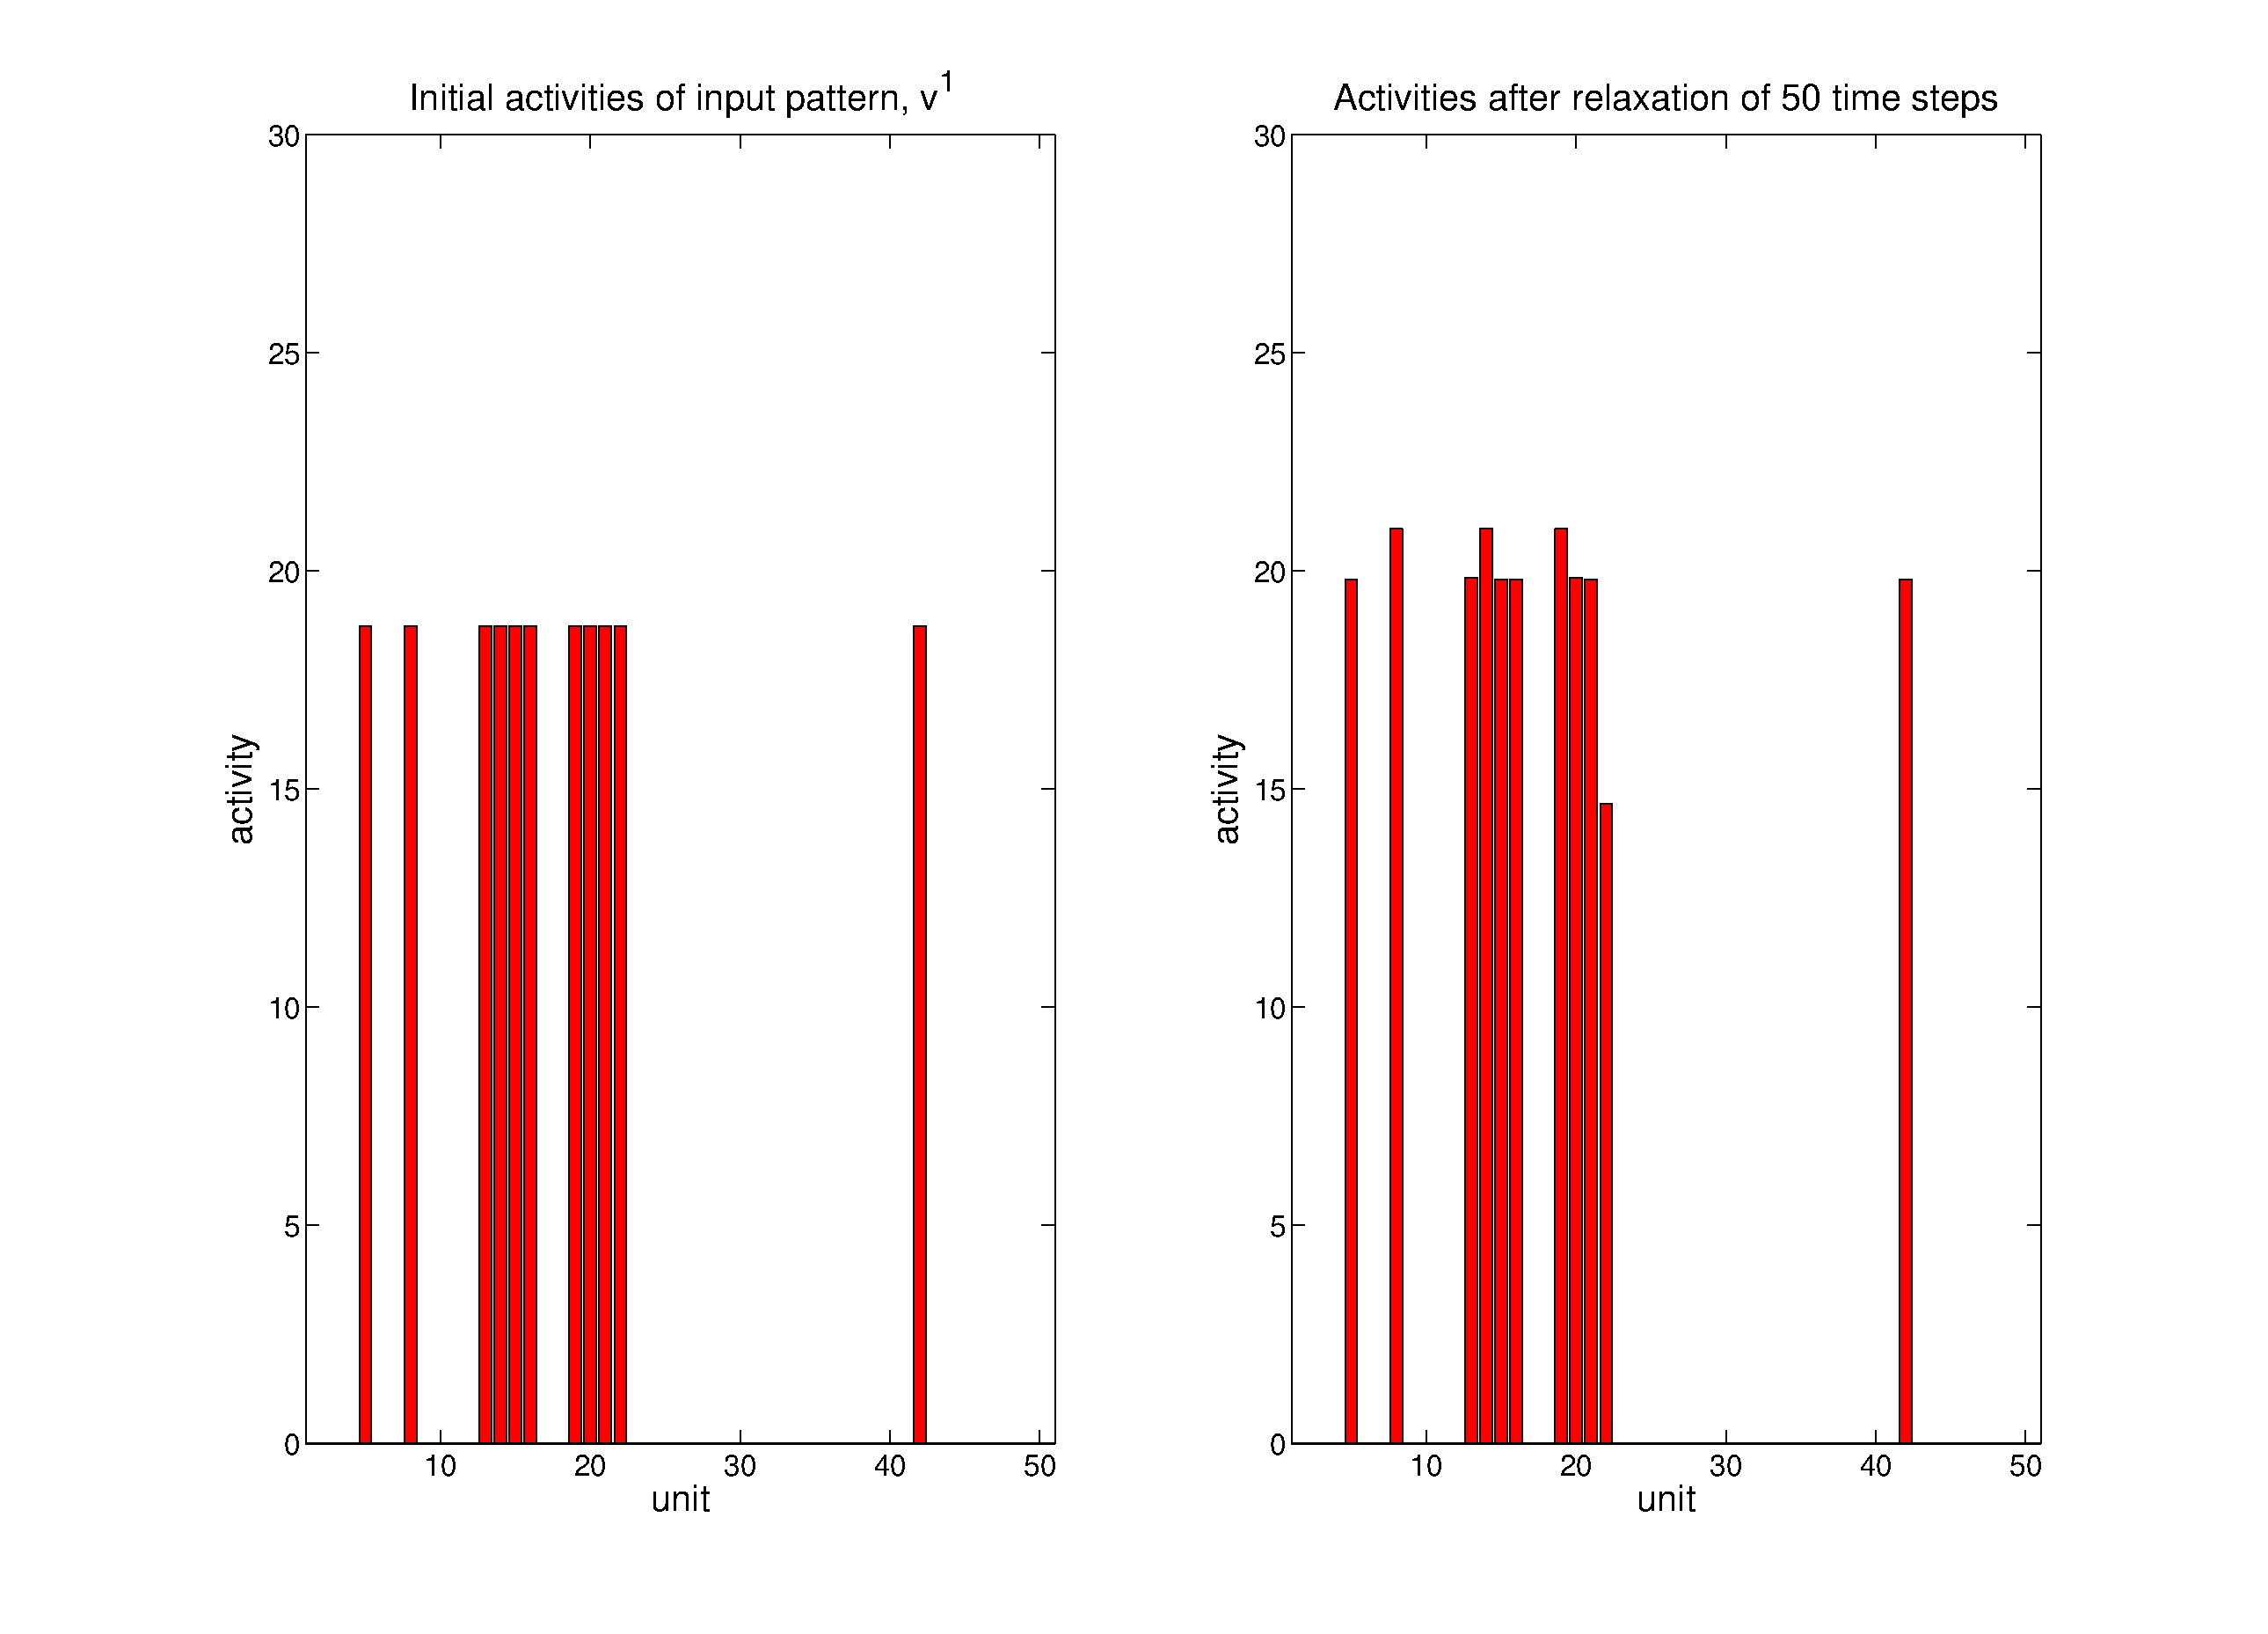
\includegraphics[width=\textwidth]{memory_pure.eps}
% tau4_M1.eps: 0x0 pixel, 300dpi, 0.00x0.00 cm, bb= -304   -42   918   834
\begin{footnotesize}
 Figure 1, How $v^1$ and its activity looks like with the provided code. 
\end{footnotesize}
\end{center}

\subsection{}
The next task is to reproduce the patterns \textbf{v}$^1$ and \textbf{v}$^2$, such that 1st pattern has only its units 18-30 being active, and 2nd pattern every 4th unit being active. Additionally the section 2.3 also asks for reproducing \textbf{v}$^3$ and \textbf{v}$^4$ freely. This is done succesfully, and the result can be seen in appendix part below. 


Let us have a look at have the first two patterns and their output activities seems to be. 

\begin{center}
\includegraphics[width=\textwidth]{memory_v1.eps}
% tau4_M1.eps: 0x0 pixel, 300dpi, 0.00x0.00 cm, bb= -304   -42   918   834
\begin{footnotesize}
 Figure 2, The memory pattern \textbf{v}$^1$ has its elements as either 0 (inactivity) or $c=18.731$ (activity) between index 18 and 31. 
\end{footnotesize}
\end{center}

\begin{center}
\includegraphics[width=\textwidth]{memory_v2.eps}
% tau4_M1.eps: 0x0 pixel, 300dpi, 0.00x0.00 cm, bb= -304   -42   918   834
\begin{footnotesize}
 Figure 3, The memory pattern \textbf{v}$^2$ as being active at each 4th  index (activity) $c=18.731$ and otherwiese 0 (activity).
\end{footnotesize}
\end{center}

\subsection{}
The self created input patterns $v^3$ and $v^4$ input patterns are given in following figures.

\begin{center}
\includegraphics[width=\textwidth, height=75mm]{memory_v3.eps}
% tau4_M1.eps: 0x0 pixel, 300dpi, 0.00x0.00 cm, bb= -304   -42   918   834
\begin{footnotesize}
 Figure 4, The memory pattern \textbf{v}$^3$ 
\end{footnotesize}
\end{center}

\begin{center}
\includegraphics[width=\textwidth, height=75mm]{memory_v4.eps}
% tau4_M1.eps: 0x0 pixel, 300dpi, 0.00x0.00 cm, bb= -304   -42   918   834
\begin{footnotesize}
 Figure 5, The memory pattern \textbf{v}$^4$ 
\end{footnotesize}
\end{center}

This sections asks for investigating the force of attraction of the corresponding fix point with respect to partial input 50 time steps by applying \textbf{v}$_c ^{t+1}=F($\textbf{M.v}$_c ^t ) $

(Please look at the provided code $memory_assign.m$ to see the output vectors of 4 initial patterns.)

Now, let us analyze the effect of strength ($\delta$) of the additional Gaussian Noise part ($\zeta$) to the input patterns. Basically, the already generated input patterns are added a noisy part with a strength. Then, the iteration is repeated again 50 times.

\begin{equation}
 \textbf{v}(t=1)=\textbf{v}^1+\zeta.\delta
\end{equation}

\begin{equation*}
 \textbf{v}(t+1)=F(\textbf{M.v}(t)) 
\end{equation*}

The effect of strength is expected as to distort the pattern. The greater the strength, the more disturbed the input pattern is. The provided plot shows statistically how the performances of calculated output patterns change by increasing strength. 

 \begin{center}
	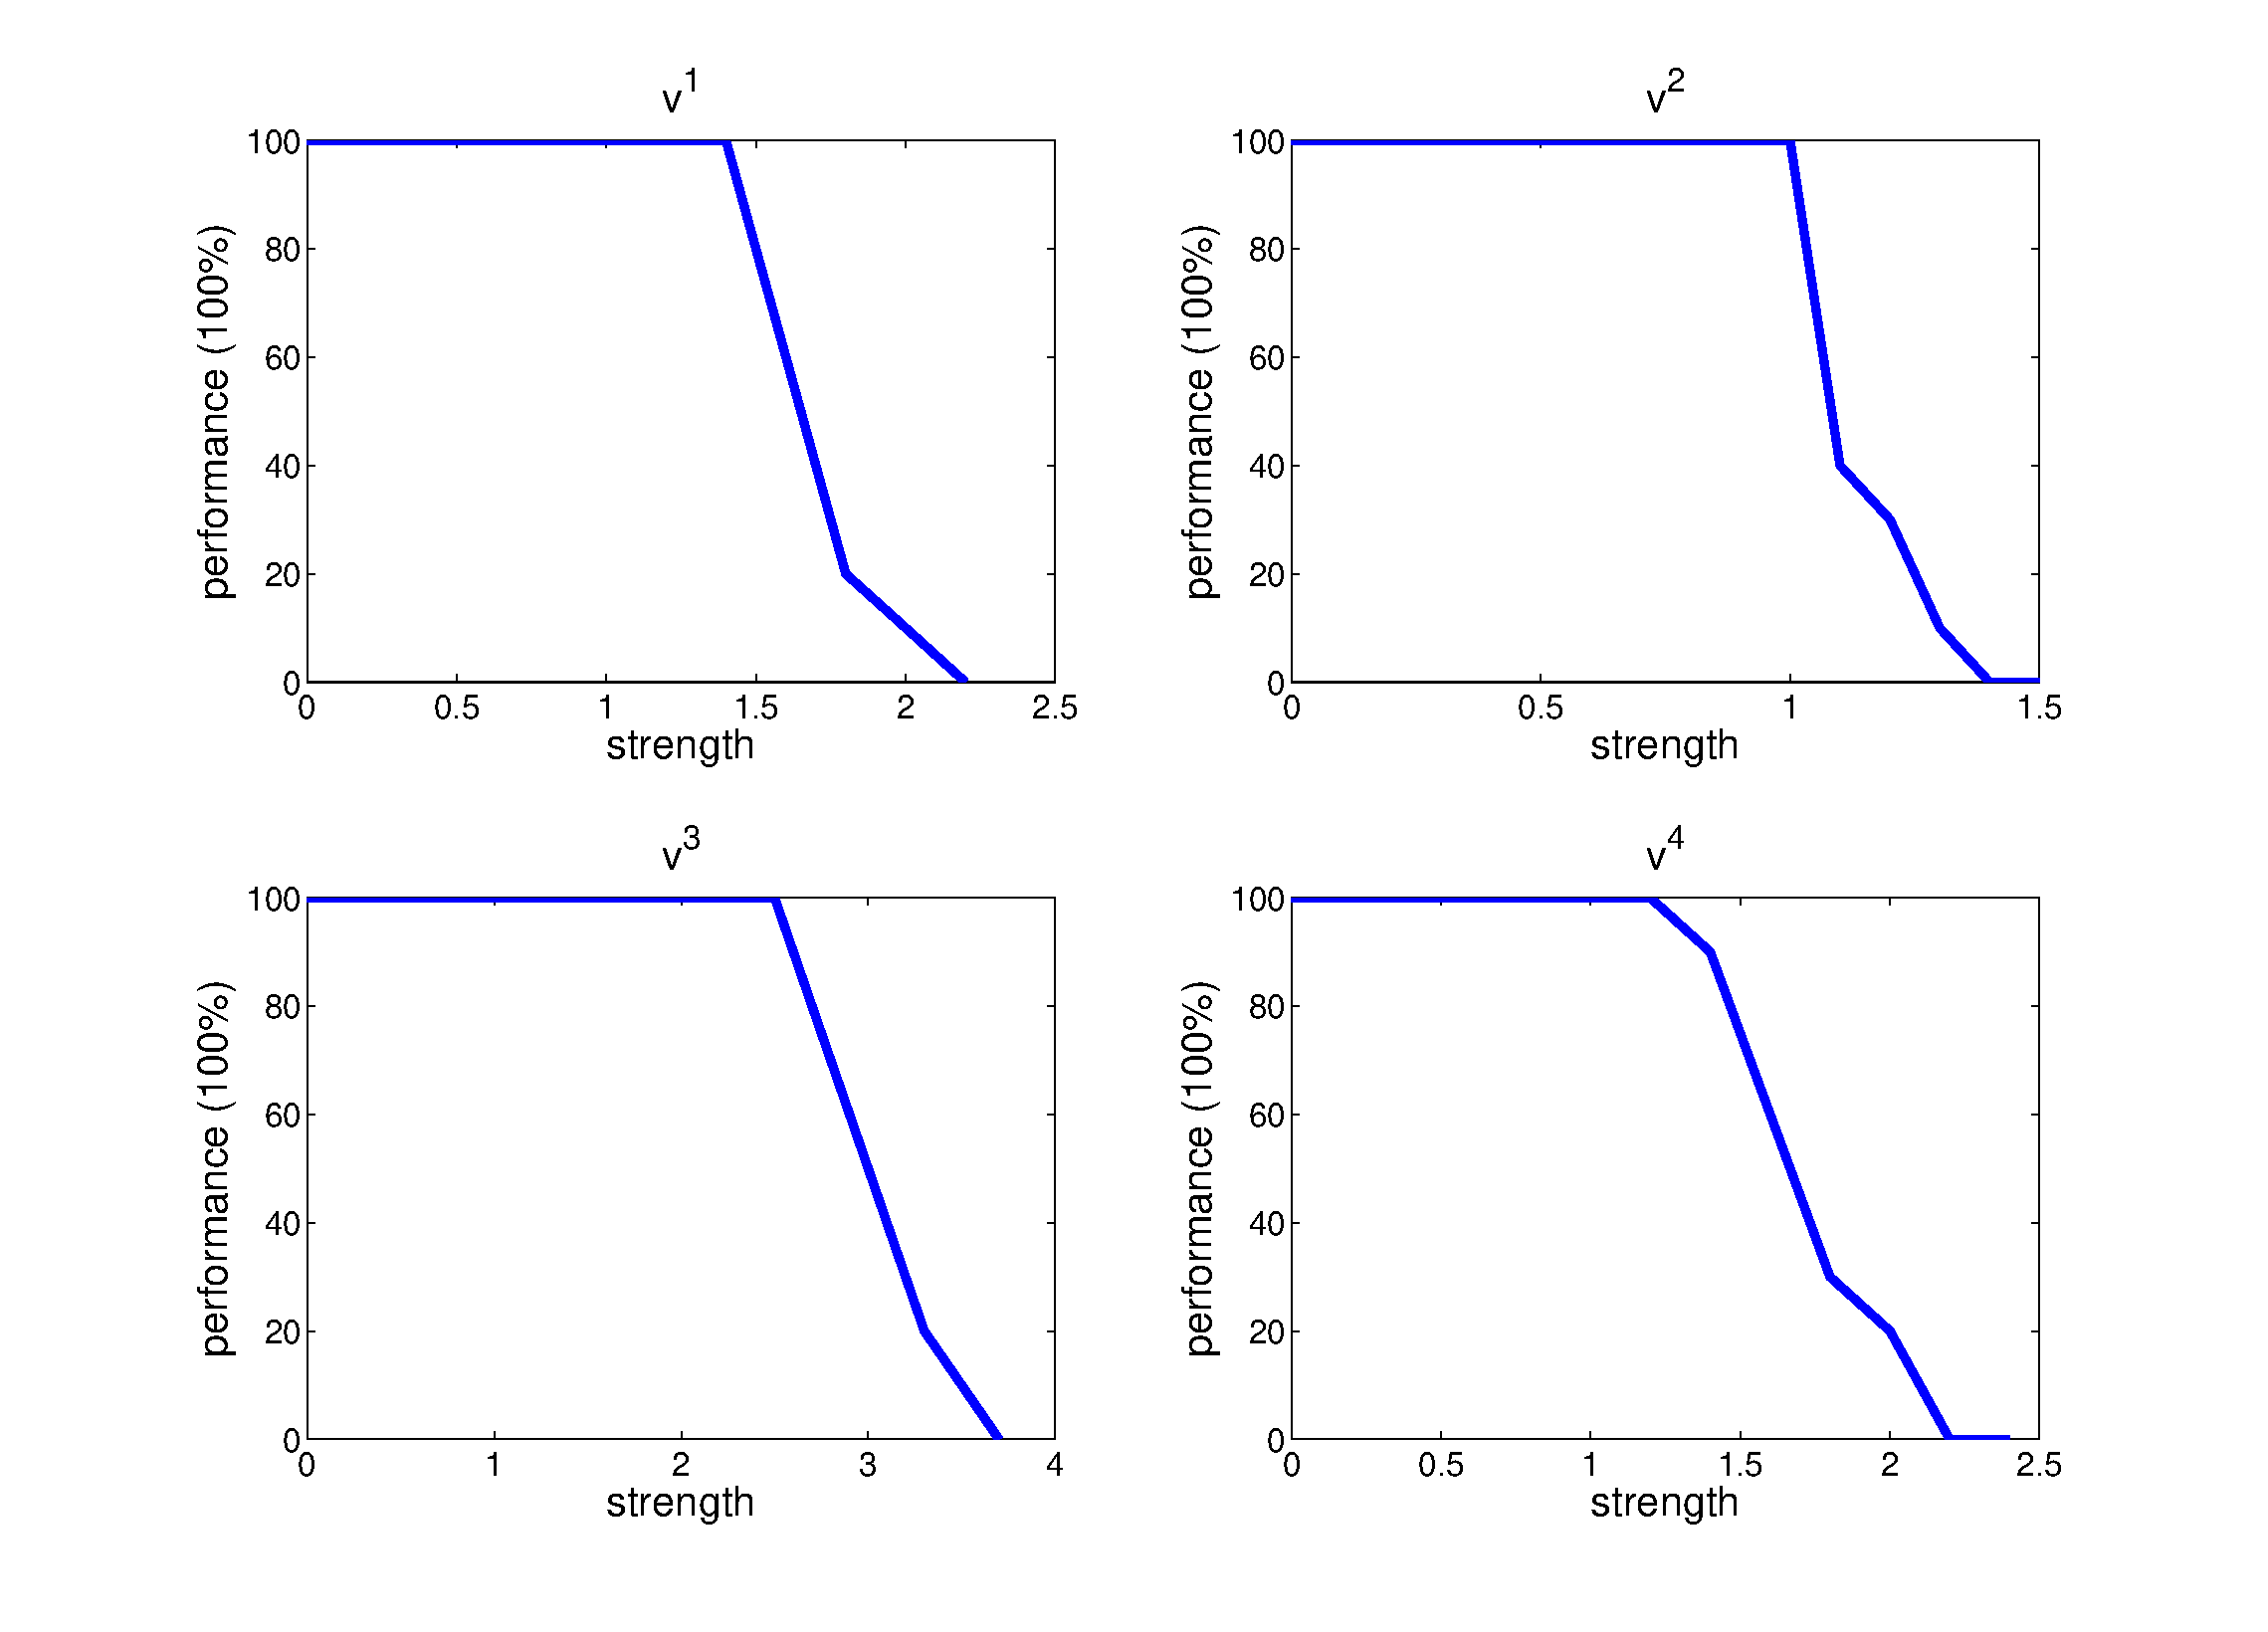
\includegraphics[width=\textwidth]{strenghts.eps}
% tau4_M1.eps: 0x0 pixel, 300dpi, 0.00x0.00 cm, bb= -304   -42   918   834
\begin{footnotesize}
 Figure 6, Performance 100 \% means that, all trials with corresponding strength value resulted as the same output \textbf{v}(t+1). Decrease if performance means the true output percentages out of total outputs.  
\end{footnotesize}
\end{center}

Figures below show exmples to distorted and undistorted input-output patterns.

 \begin{center}
	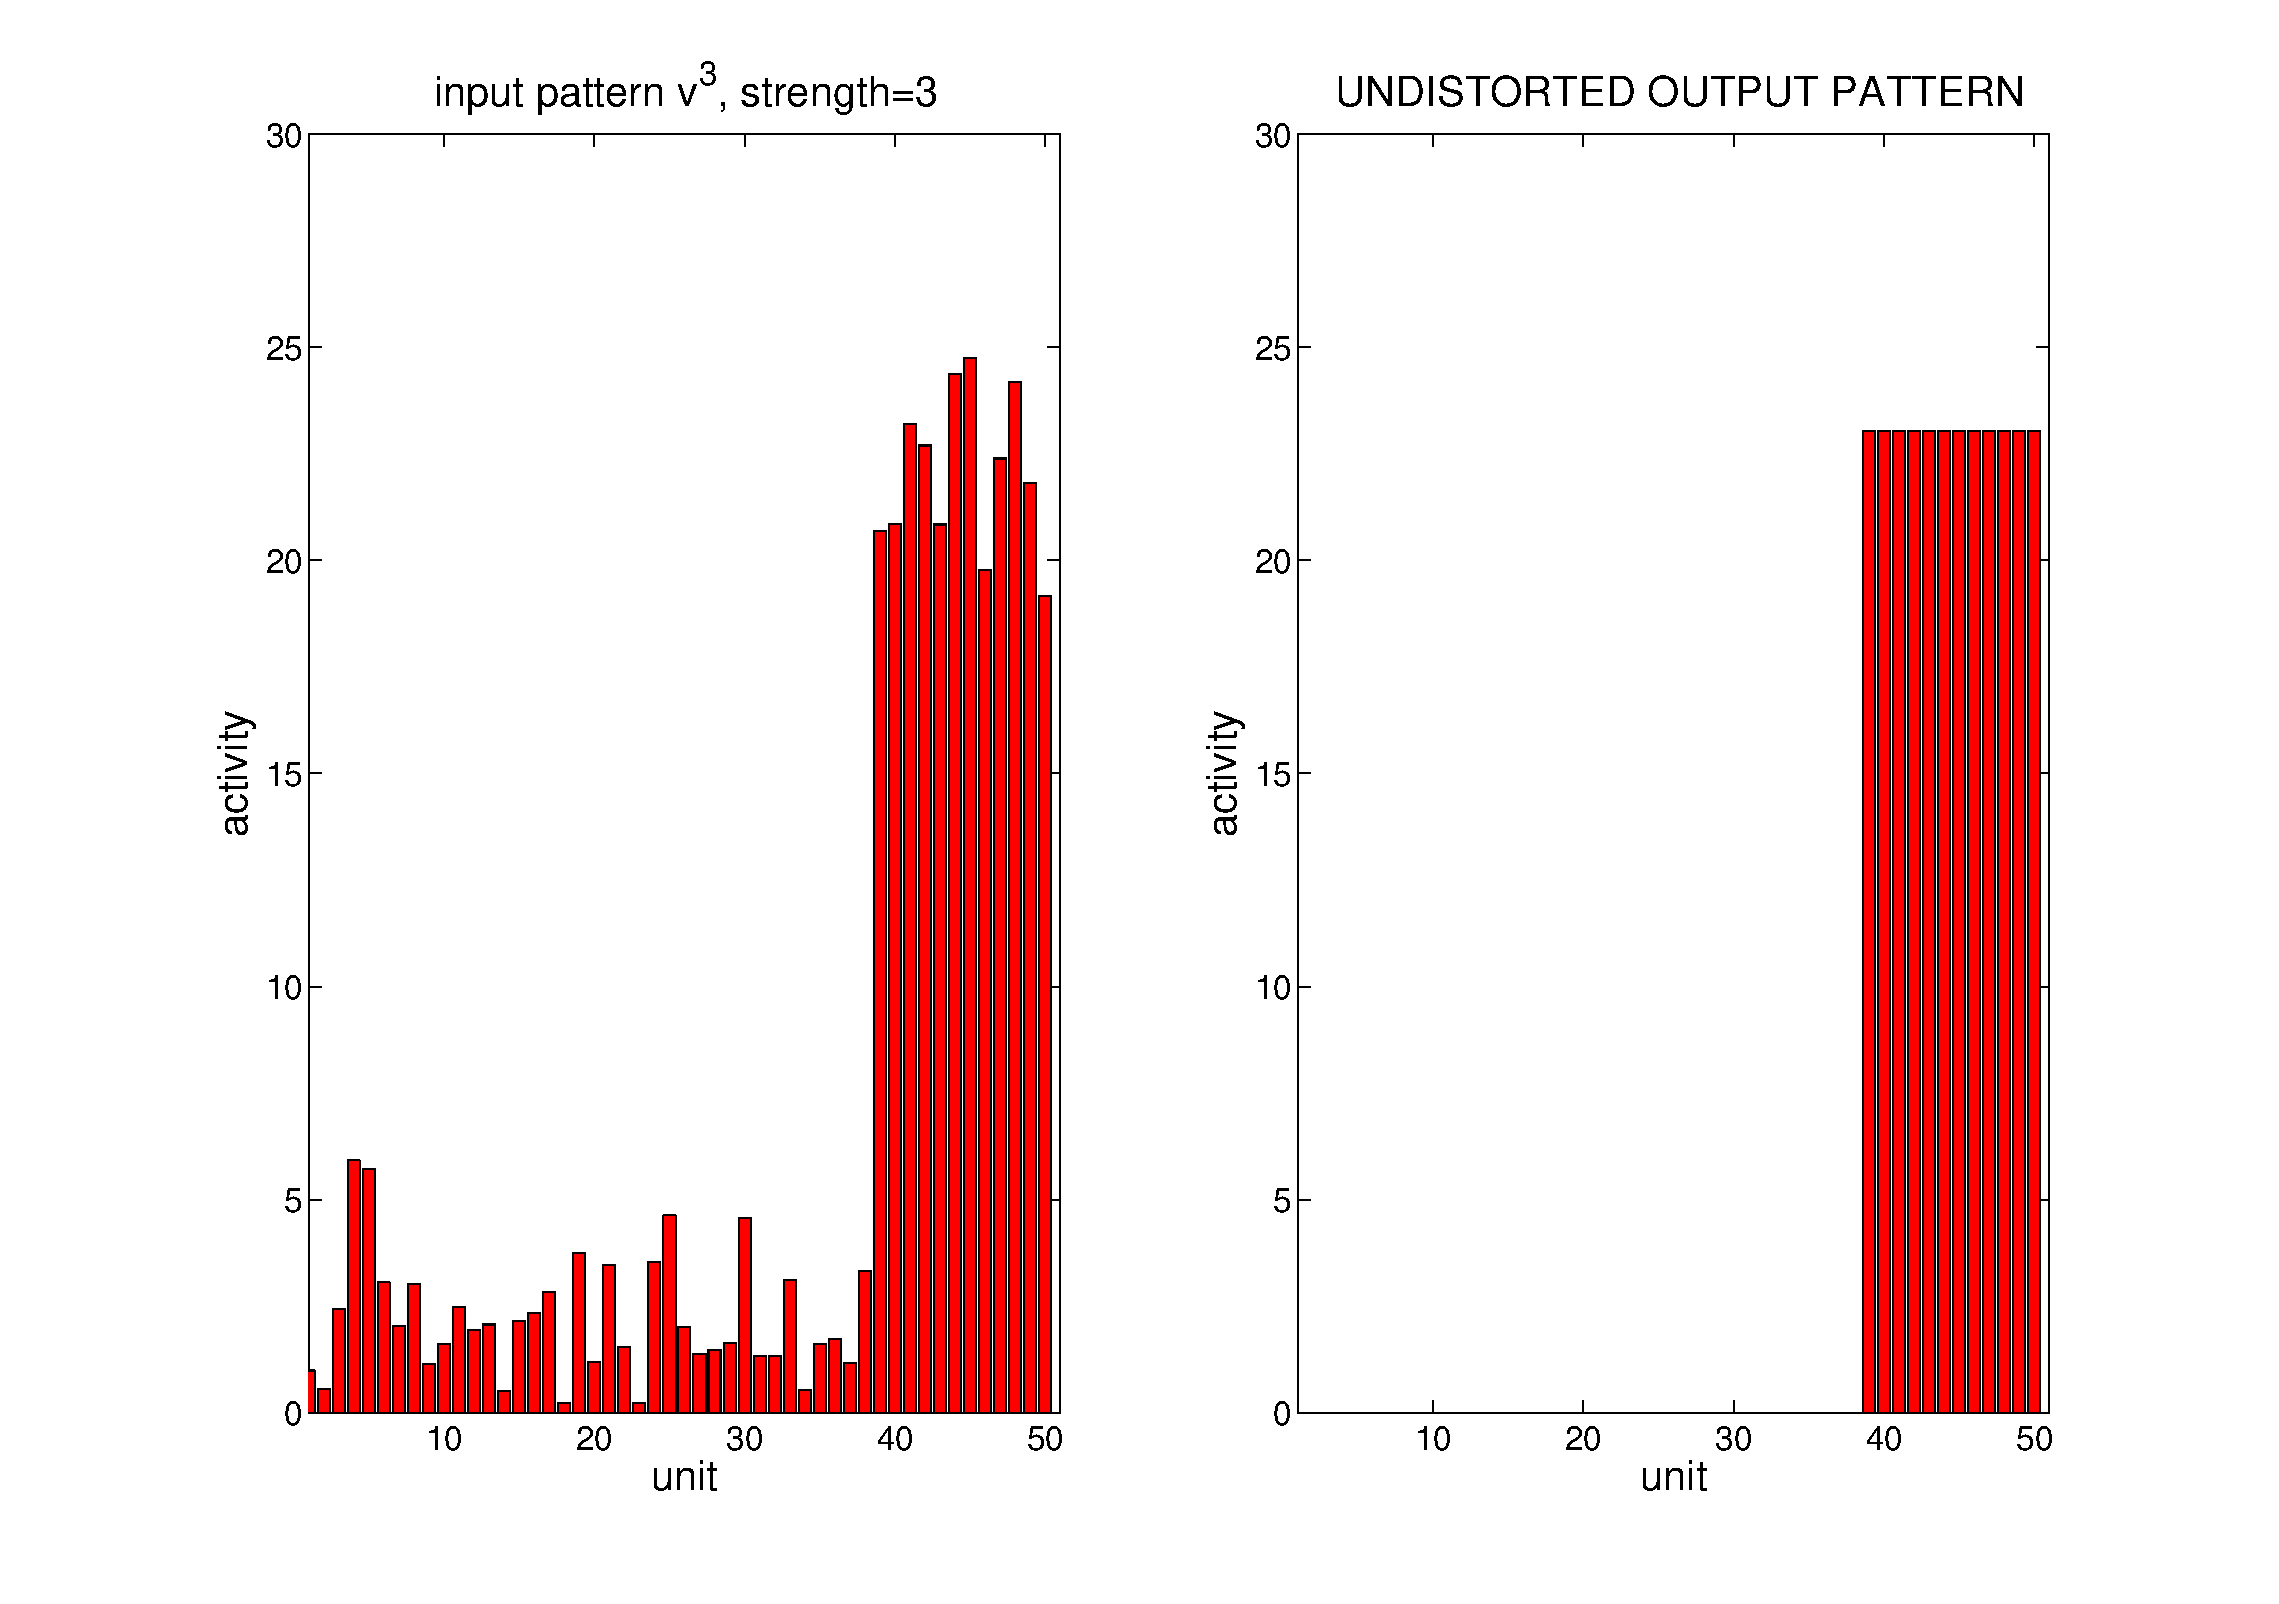
\includegraphics[width=\textwidth]{undistorted.eps}
% tau4_M1.eps: 0x0 pixel, 300dpi, 0.00x0.00 cm, bb= -304   -42   918   834
\begin{footnotesize}
 Figure 7, Although the input pattern is highly distorted, the output pattern might still stay undisturbed. \end{footnotesize}
\end{center}


 \begin{center}
	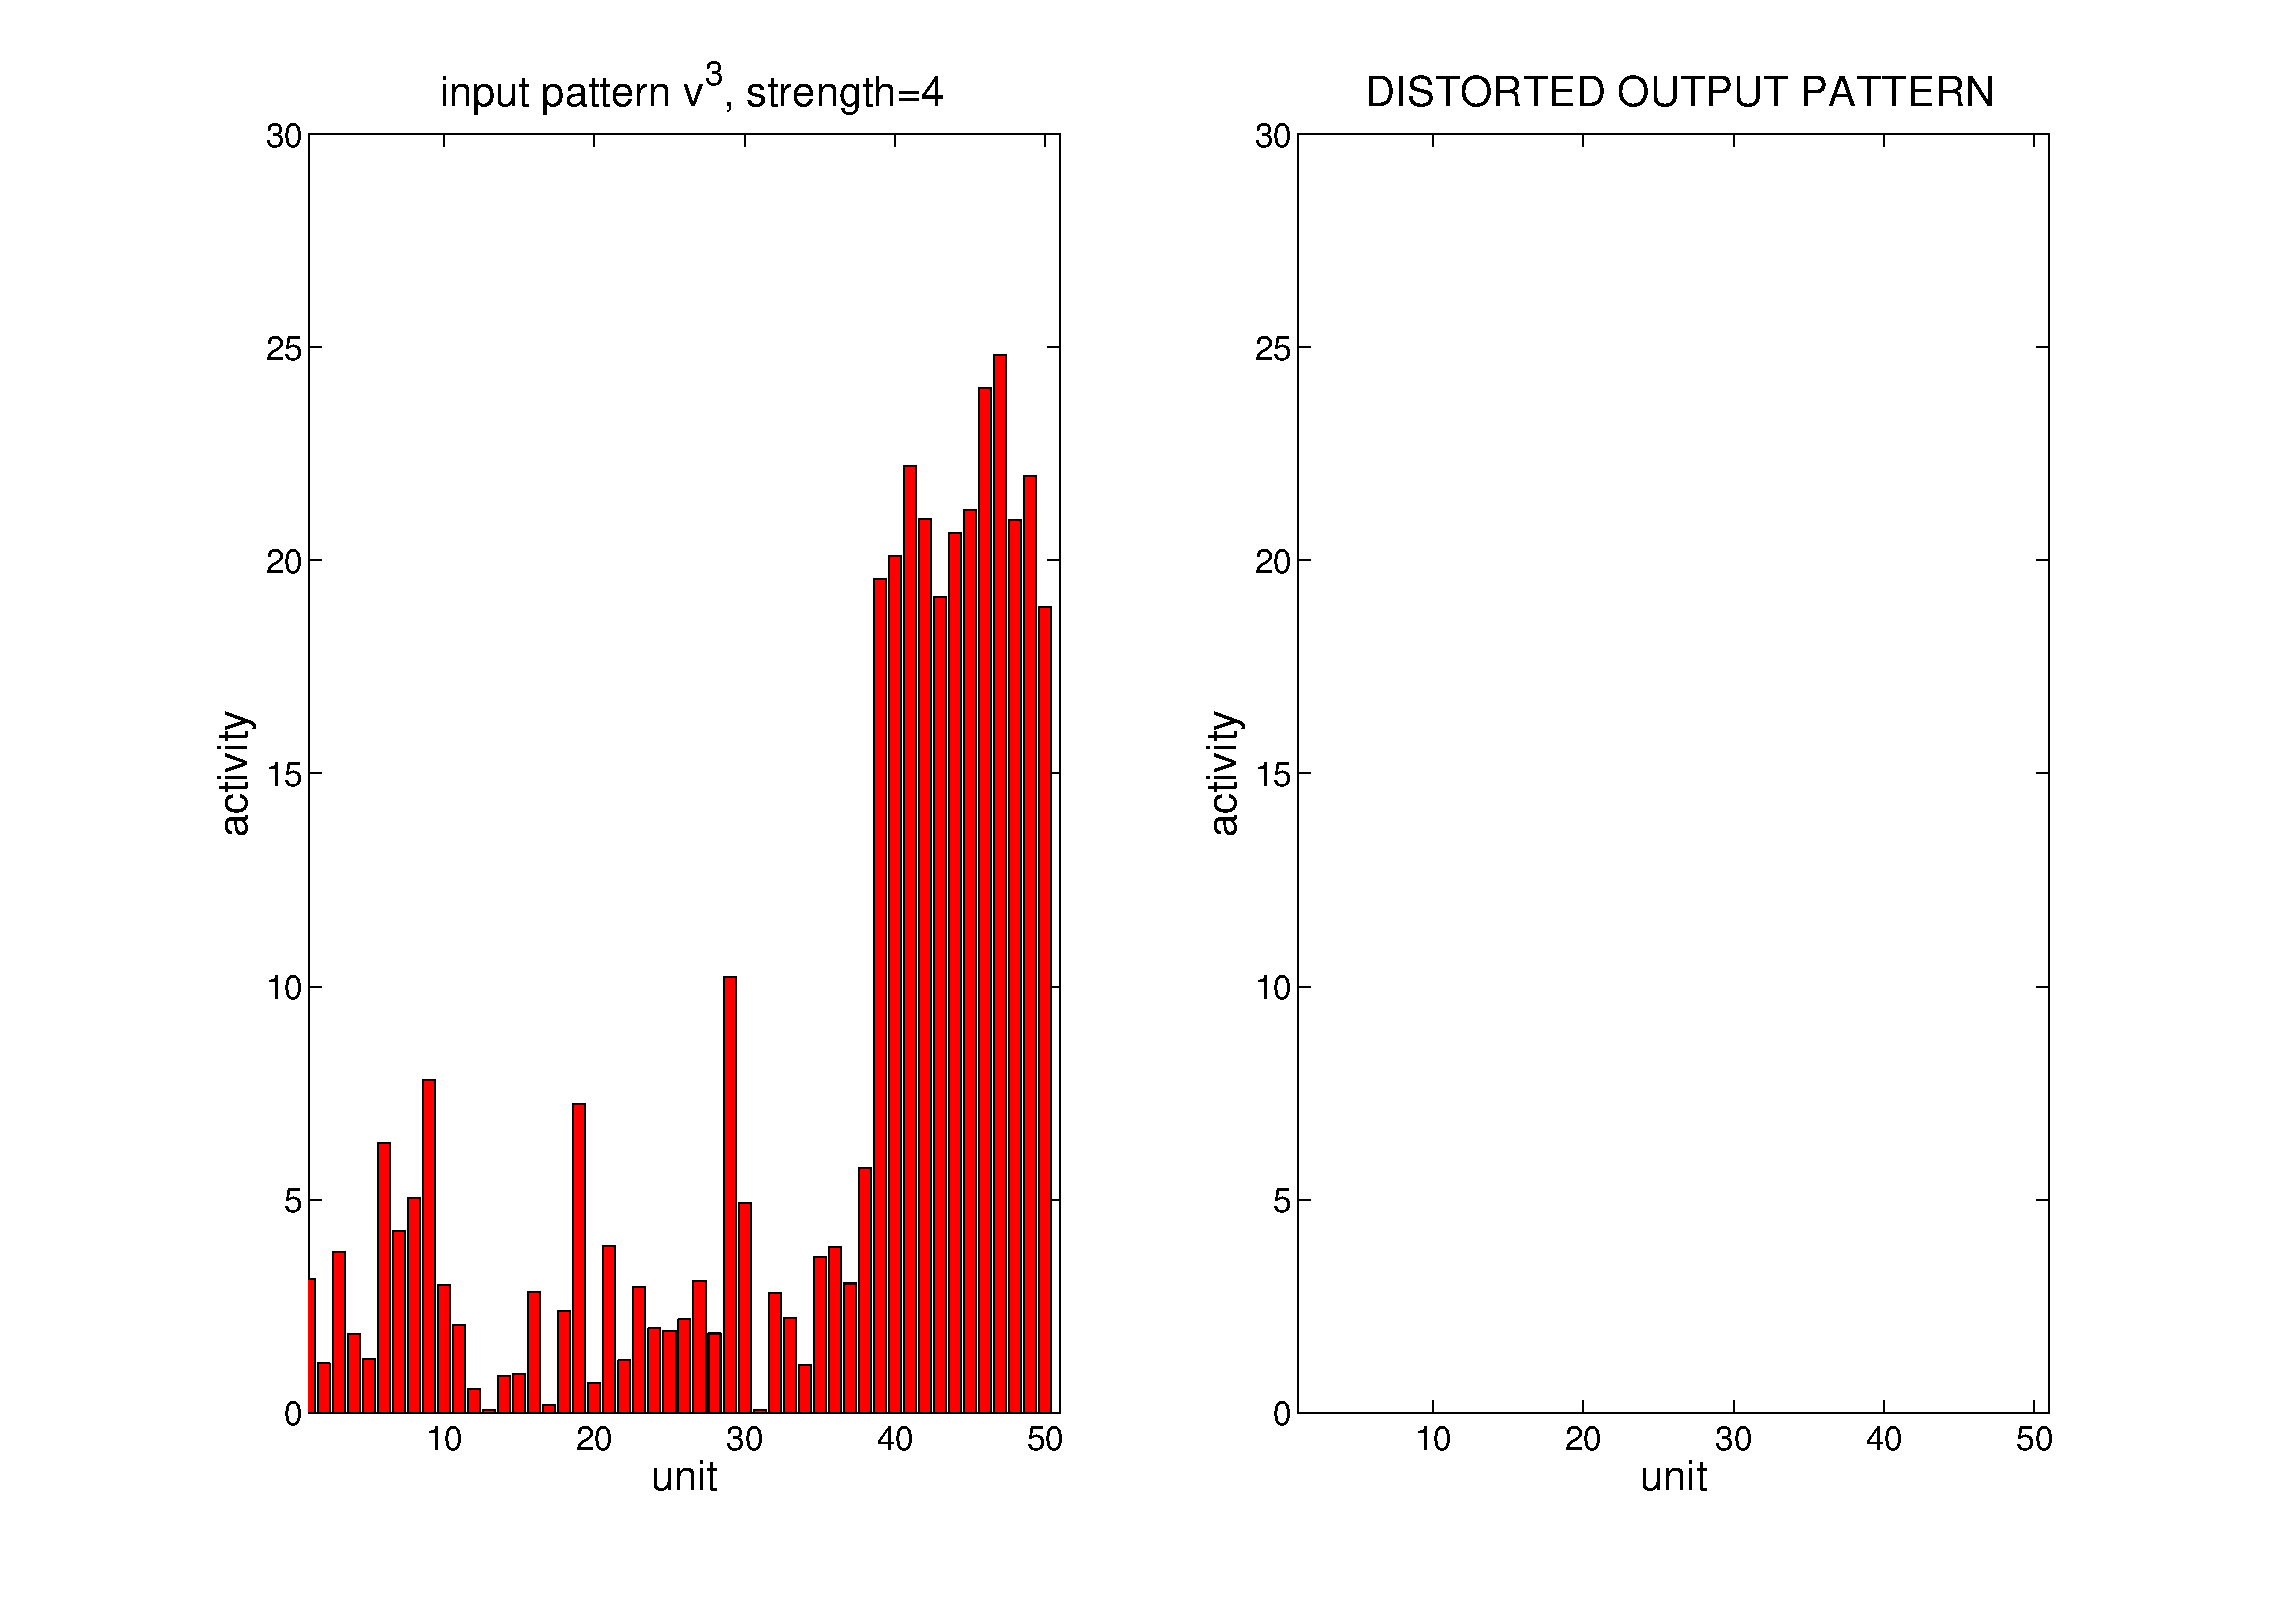
\includegraphics[width=\textwidth]{distorted.eps}
% tau4_M1.eps: 0x0 pixel, 300dpi, 0.00x0.00 cm, bb= -304   -42   918   834
\begin{footnotesize}
 Figure 8, The input pattern is distorted this time by a higher noise strength, and the output seems to be distorted too. \end{footnotesize}
\end{center}

\subsection{Optinal Task}

What is the influence of $\alpha$ to the input and output patterns? Let us look at how $c$ changes wiht the different $\alpha$ values as seen in Table 1.\newline

\begin{center}
\begin{footnotesize}Table 1 
 \end{footnotesize} 
\end{center}

\begin{center}
 \begin{tabular} {l || c|c|c| c|c|c| c|c|c| r }
$\alpha$ & 0 & 0.2 & 0.4 & 0.6 & 0.8 & 1 & 2 & 4 & 6 &8 \\ \hline
 c & 26.30 & 19.88 & 19.95 & 13.31 & 11.42 & 9.99 & 6.15 & 3.48&2.43&1.83\\
  
 \end{tabular}

\end{center}

$\alpha$ represents the probability of assigning an activation into the input vector \textbf{v}. In other words $1-\alpha$ is the probability of assigning inactivation (or 0) into the input pattern. It is also called as the "sparseness" of the memory pattern, it determines how mony different patterns one can get. If the pattern is sparser, it can store more inside but it affects the output negatively, so that it leads to a less information content. Table 1 shows that the bigger the $\alpha$ is, the less the $c$. Actually, since $\alpha$ stands for the probability, it may be more reasonable to consider the values between 0 and 1 for it. If we say that, the input pattern has 50 elements ($N_v$), the distribution of activitity is related to the binomial distribution $\sim$B($N_v$,$k\sim(\alpha)$). To create the highest activity pattern, $k$ should be 25 and corresponding $\alpha$ is 0.5 (this is the hint given by tutorial instructor). Let's look the figure below for $\alpha=0.5$.

 \begin{center}
	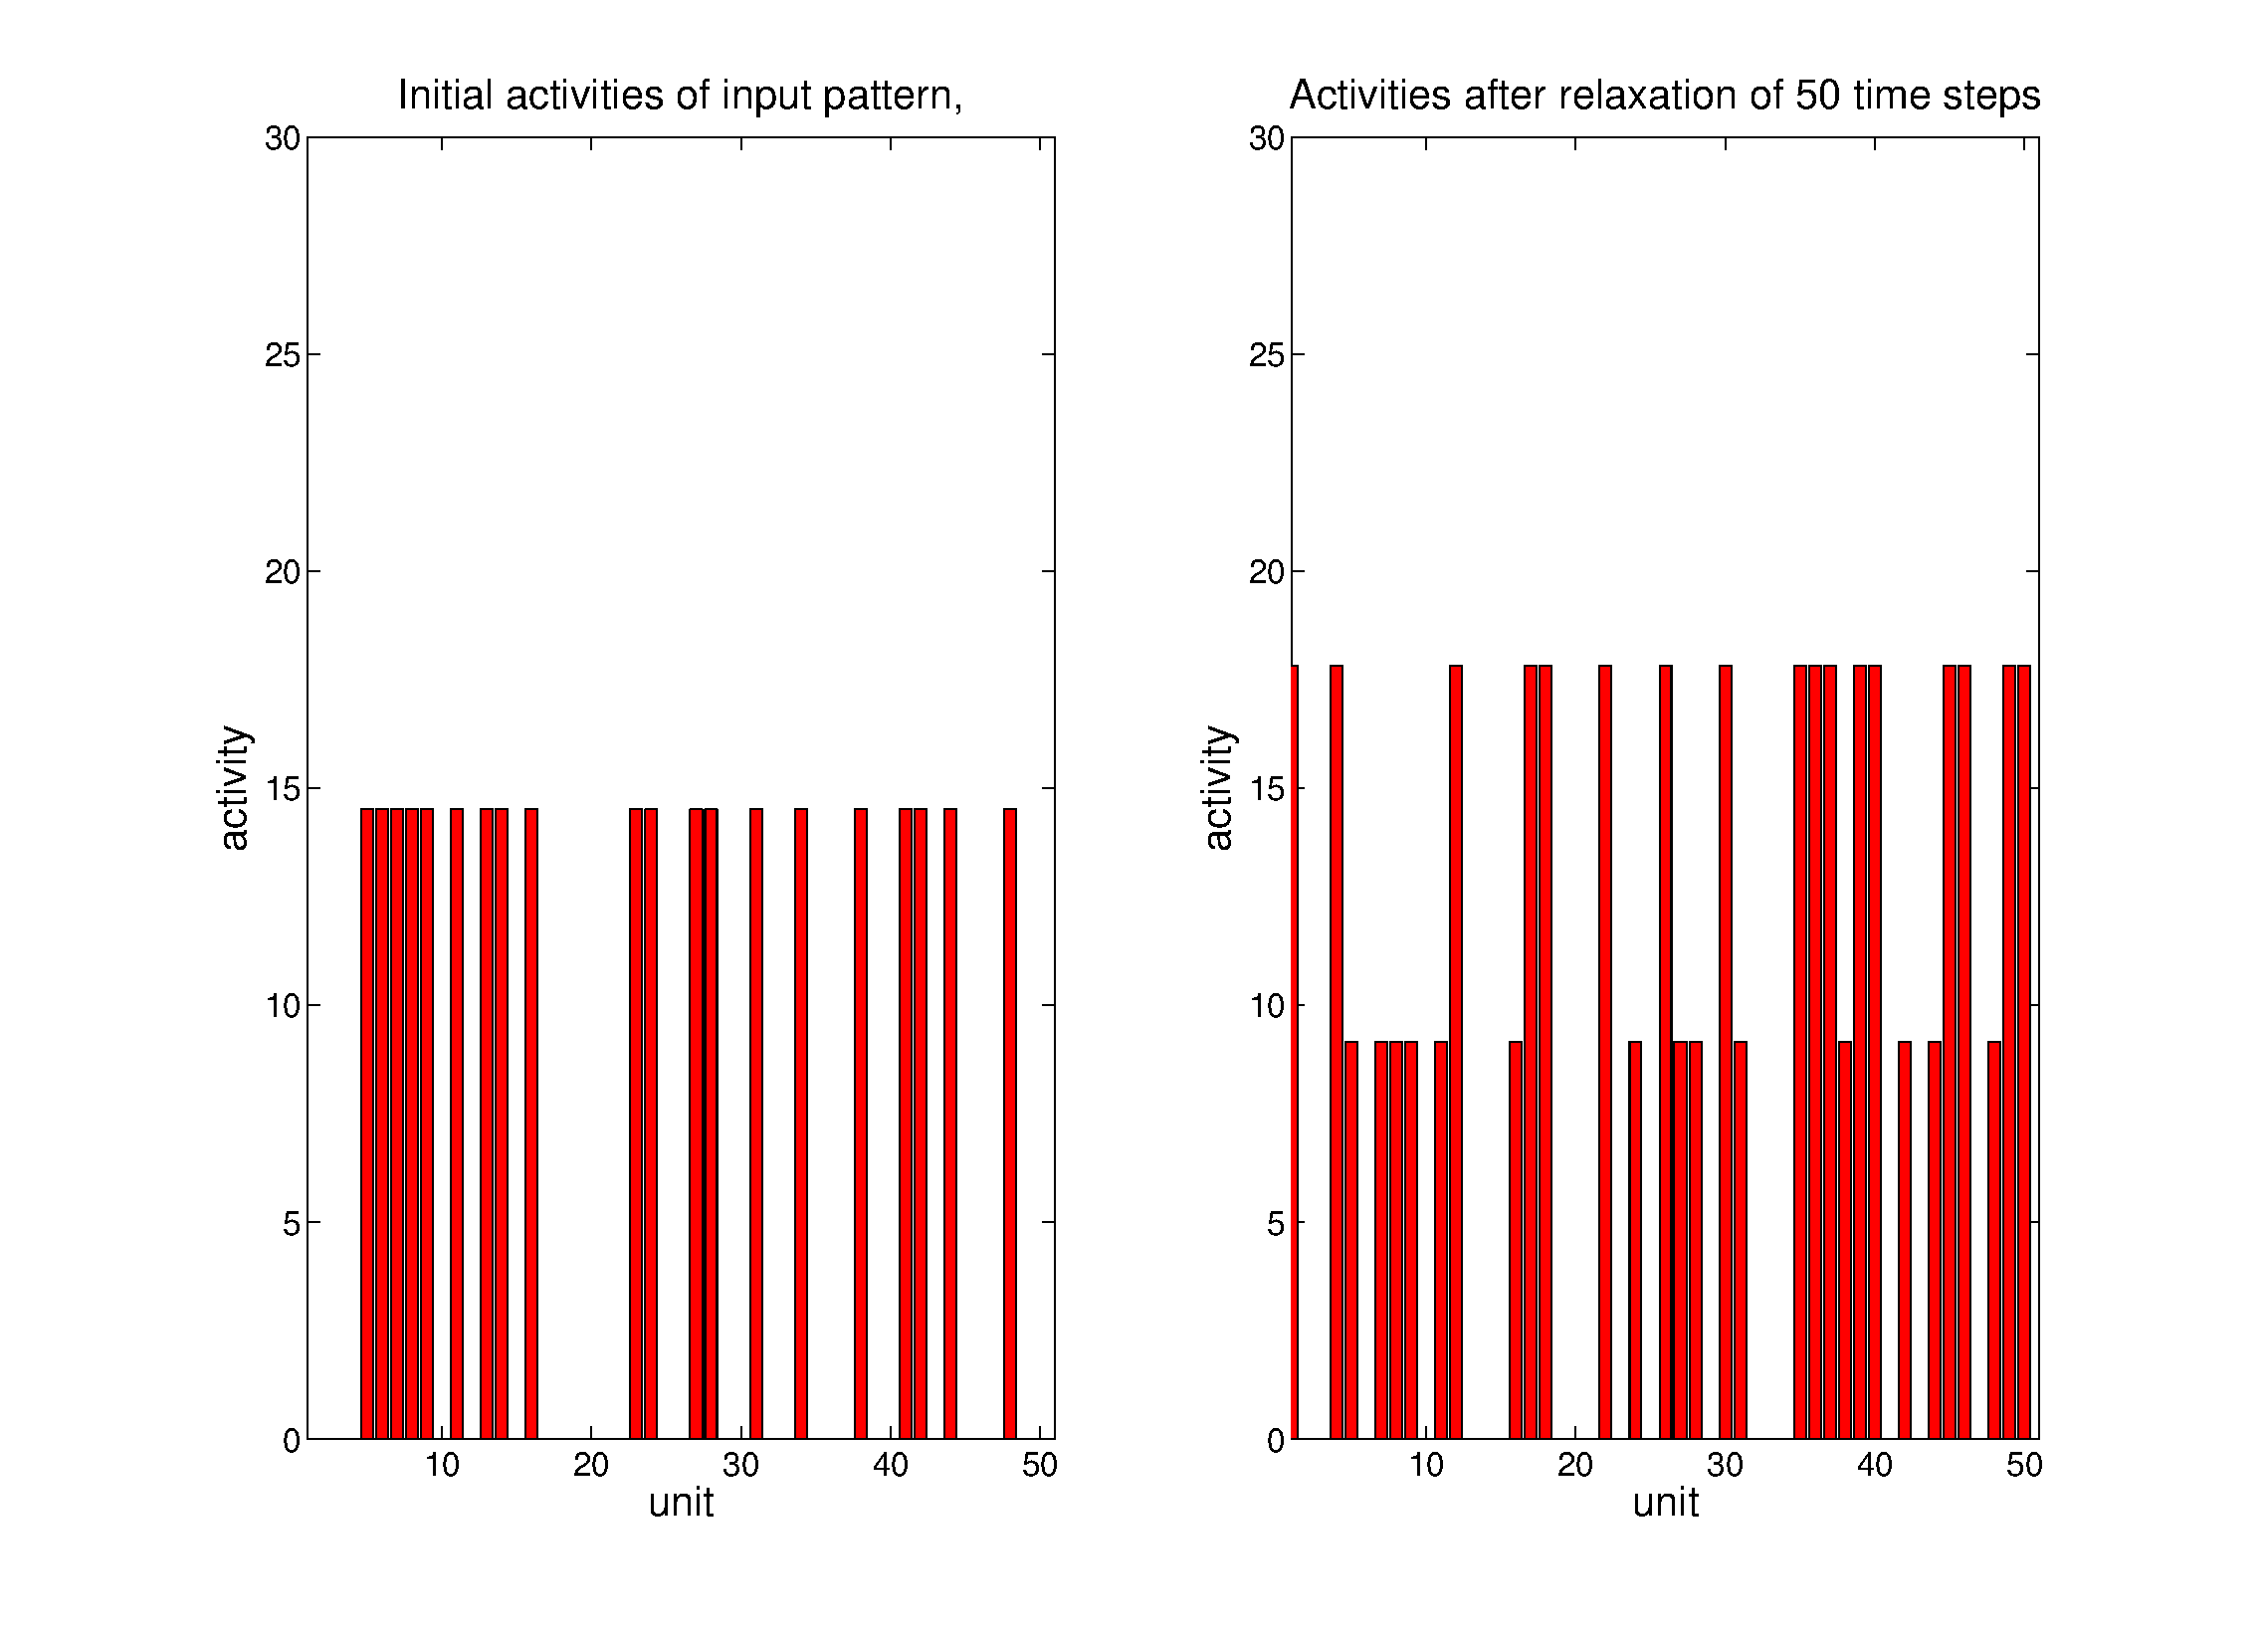
\includegraphics[width=\textwidth]{alpha1.eps}
% tau4_M1.eps: 0x0 pixel, 300dpi, 0.00x0.00 cm, bb= -304   -42   918   834
\begin{footnotesize}
 Figure 9, The input pattern \textbf{v}$^1$ with no distortion (strength=0), $\alpha=0.5$ \end{footnotesize}
\end{center}

However, I found the activity patterns maximum around $\alpha=0.7$ as seen below. 

 \begin{center}
	\includegraphics[width=\textwidth]{alpha2.eps}
% tau4_M1.eps: 0x0 pixel, 300dpi, 0.00x0.00 cm, bb= -304   -42   918   834
\begin{footnotesize}
 Figure 10, The input pattern \textbf{v}$^1$ without any distortion , $\alpha=0.7$. In comparison to figure 9, $c$ decreases, however output activity increases. \end{footnotesize}
\end{center} 

The maximum number of possible memory patterns is by the way proportional to the length of input patterns.

\begin{equation}
 N_{mem} \propto N_{v}
\end{equation}


\section{Appendix}

	\begin{verbatim}
 
K>> [vn(:,1) vn(:,2) vn(:,3) vn(:,4)]

ans =

         0         0         0         0
         0         0         0         0
         0         0         0   18.7310
         0   18.7310         0         0
         0         0         0         0
         0         0         0   18.7310
         0         0         0         0
         0   18.7310         0         0
         0         0         0   18.7310
         0         0         0         0
         0         0         0         0
         0   18.7310         0   18.7310
         0         0         0         0
         0         0         0         0
         0         0         0   18.7310
         0   18.7310         0         0
         0         0         0         0
         0         0         0   18.7310
   18.7310         0         0         0
   18.7310   18.7310         0         0
   18.7310         0         0   18.7310
   18.7310         0         0         0
   18.7310         0         0         0
   18.7310   18.7310         0   18.7310
   18.7310         0         0         0
   18.7310         0         0         0
   18.7310         0         0   18.7310
   18.7310   18.7310         0         0
   18.7310         0         0         0
   18.7310         0         0   18.7310
         0         0         0         0
         0   18.7310         0         0
         0         0         0   18.7310
         0         0         0         0
         0         0         0         0
         0   18.7310         0   18.7310
         0         0         0         0
         0         0         0         0
         0         0   18.7310         0
         0   18.7310   18.7310         0
         0         0   18.7310         0
         0         0   18.7310         0
         0         0   18.7310         0
         0   18.7310   18.7310         0
         0         0   18.7310         0
         0         0   18.7310         0
         0         0   18.7310         0
         0   18.7310   18.7310         0
         0         0   18.7310         0
         0         0   18.7310         0

	\end{verbatim}


\end{document}
